\chapter{シミュレーション}
\label{chap::simulation}
\section{$\alpha$線源での測定}
${}^{241}{\rm Am}$ $\alpha$線源を用いて測定を行った。

\subsection{各検出ガスにおけるドリフトスピード}
電子のドリフトスピードを線源によって得られるトラックから求める。
図\ref{pic::collimator}のような線源のコリメータを用いる。
このコリメータはアクリルで作られており、1つの0${}^{\circ}$、4つの30${}^{\circ}$の穴が開いている。
\begin{figure}
  \centering
  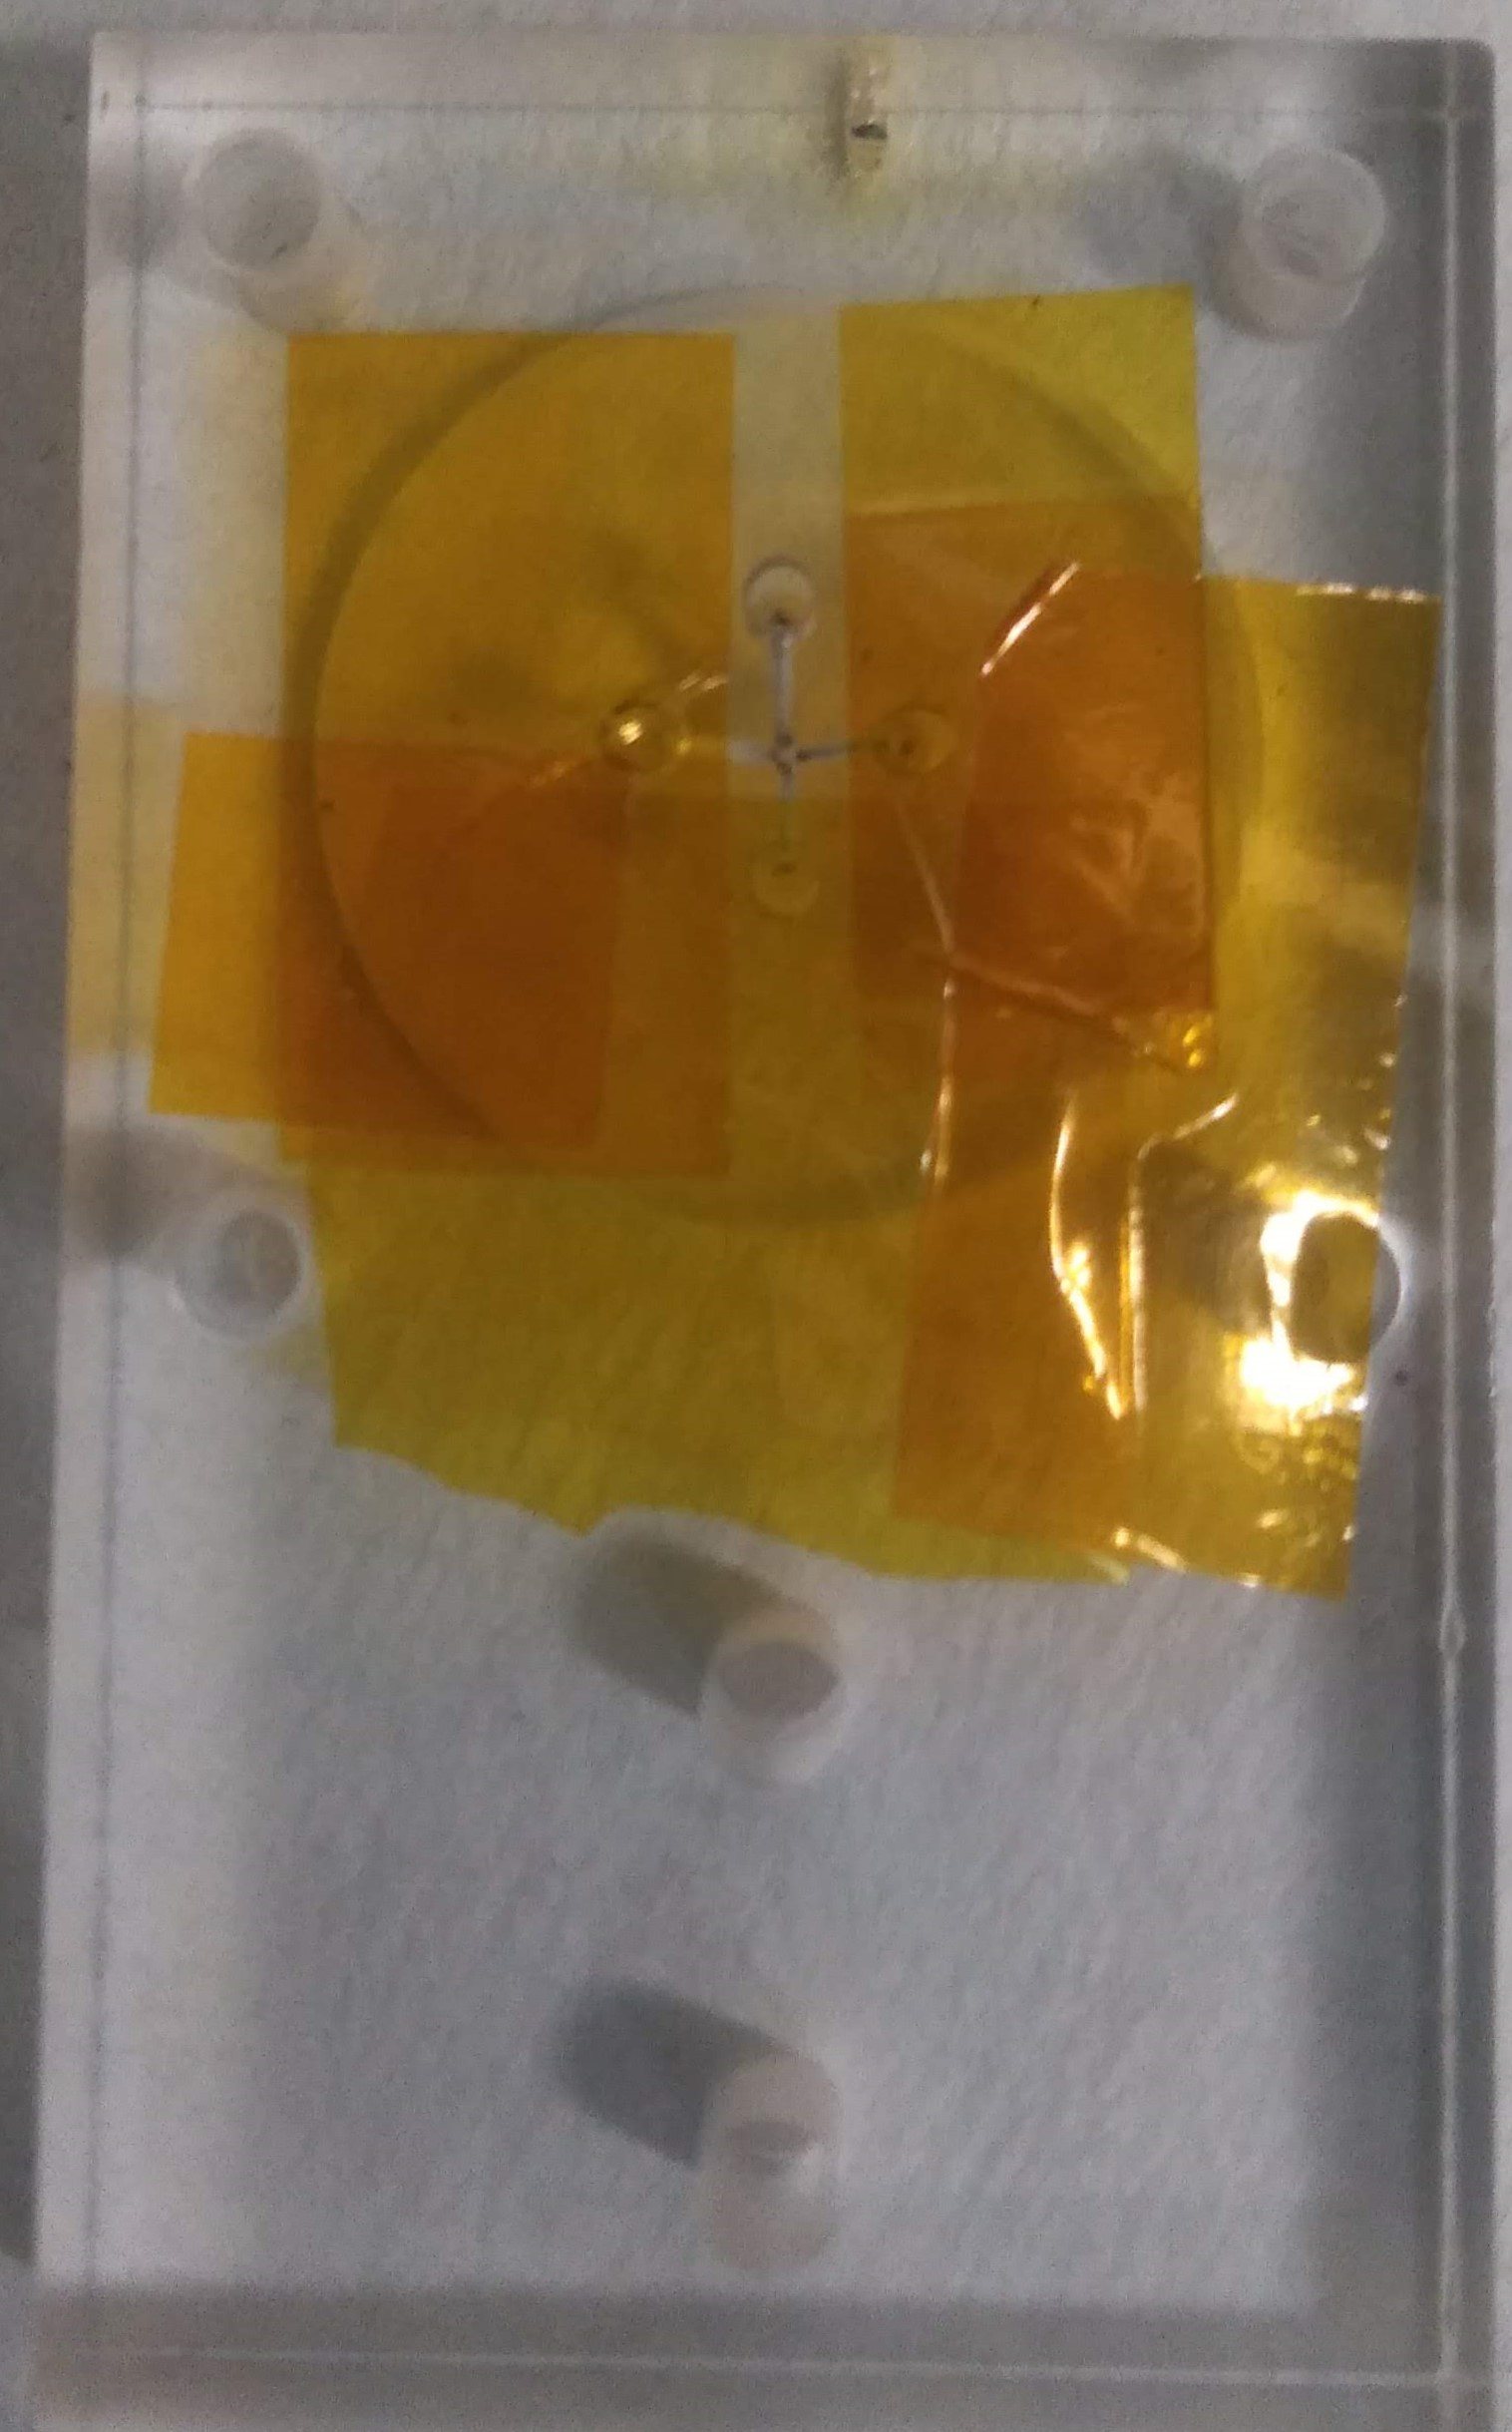
\includegraphics[clip, height=0.7\columnwidth, angle=90]{pic/IMG_20191023_145443_trmd.jpg}
  \caption[線源コリメータ。]
          {線源コリメータ。中央に0${}^{\circ}$、上下左右に30${}^{\circ}$の穴が開いている。}
  \label{pic::collimator}  
\end{figure}
このコリメータを用いることで$\alpha$線を30${}^{\circ}$の方向に限定することができる。
\begin{figure}
  \centering
  \begin{minipage}{0.45\columnwidth}
    \centering
    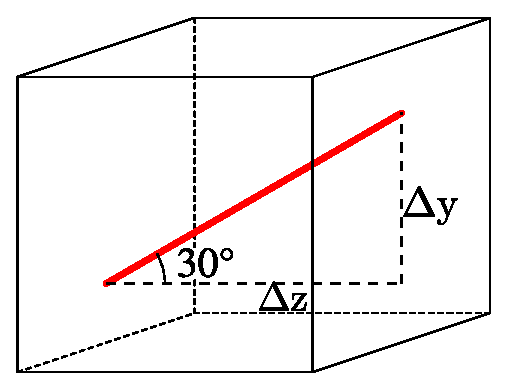
\includegraphics[clip, width=0.9\columnwidth]{eps/drift_v_source.eps}
  \end{minipage}
  \begin{minipage}{0.45\columnwidth}
    \centering
    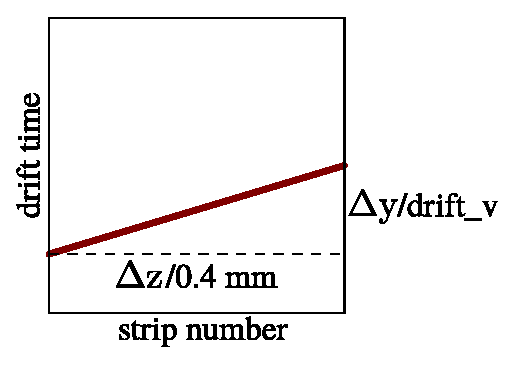
\includegraphics[clip, width=0.9\columnwidth]{eps/drift_v_image.eps}
  \end{minipage}
  \caption[30${}^{\circ}$に方向を限定した$\alpha$線と取得される画像データのイメージ。]
          {30${}^{\circ}$に方向を限定した$\alpha$線 (左) と取得される画像データ (右) のイメージ。}
  \label{fig::drift_v_image}
\end{figure}
図\ref{fig::drift_v_image}の右のようにドリフト方向に$\Delta y$、それと垂直な方向に$\Delta z$移動するとき、
\begin{equation}
  \Delta y = \tan(30^{\circ})\Delta z \label{eq::deltay_deltaz}
\end{equation}
となる。
取得されたデータのトラックが横方向に$\Delta strip$、縦方向に$\Delta t$、
ドリフトスピードを$drift\_v$とすると、
\begin{align}
  \frac{\Delta z}{0.4 {\rm mm}} & = \Delta strip \label{eq::deltaz}\\
  \frac{\Delta y}{drift\_v} & = \Delta t \label{eq::deltay}
\end{align}
式 (\ref{eq::deltay_deltaz}, \ref{eq::deltaz}, \ref{eq::deltay}) より
\begin{equation}
  drift\_v = \frac{\tan(30^{\circ})~\Delta strip\times0.4~{\rm mm}}{\Delta t}
\end{equation}
とドリフトスピードが求まる。

$\alpha$線源を用いて測定したドリフトスピードとMagboltz との比較を
図\ref{fig::drift_v_CH4}, \ref{fig::drift_v_CH4_H2}, \ref{fig::drift_v_CH4_He},
\ref{fig::drift_v_iC4H10_H2}, \ref{fig::drift_v_iC4H10_He}に示す。
\begin{figure}
  \centering
  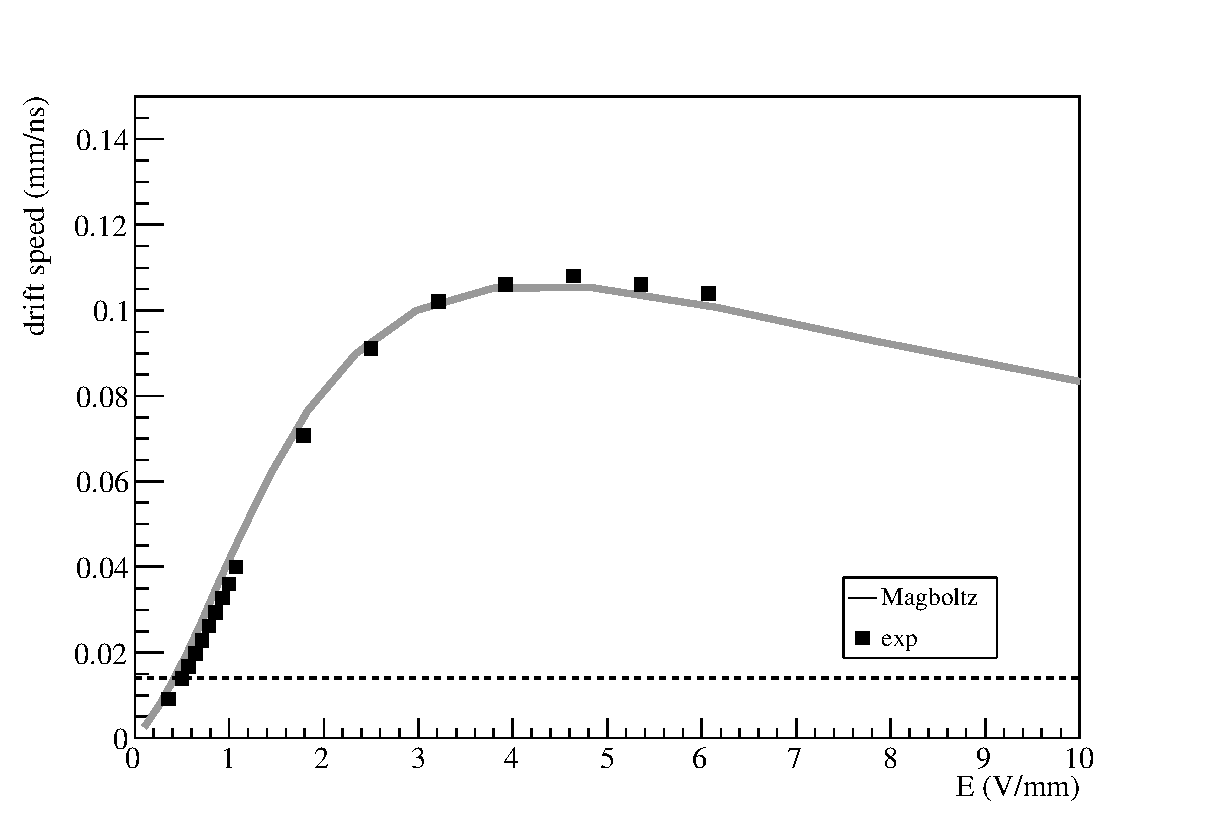
\includegraphics[clip, width=0.9\columnwidth]{eps/drift_v_CH4.eps}
  \caption[検出ガスに${\rm CH_{4}}$を用いたときのドリフトスピードの電場依存性。]
          {検出ガスに${\rm CH_{4}}$を用いたときのドリフトスピードの電場依存性。
            図中の点線は0.014 mm/ns を示す。}
  \label{fig::drift_v_CH4}
%  \includegraphics[clip, width=0.7\columnwidth]{eps/drift_v_CH4_H2.eps}
  \caption{}
  \label{fig::drift_v_CH4_H2}
%  \includegraphics[clip, width=0.7\columnwidth]{eps/drift_v_CH4_He.eps}
  \caption{}
  \label{fig::drift_v_CH4_He}
  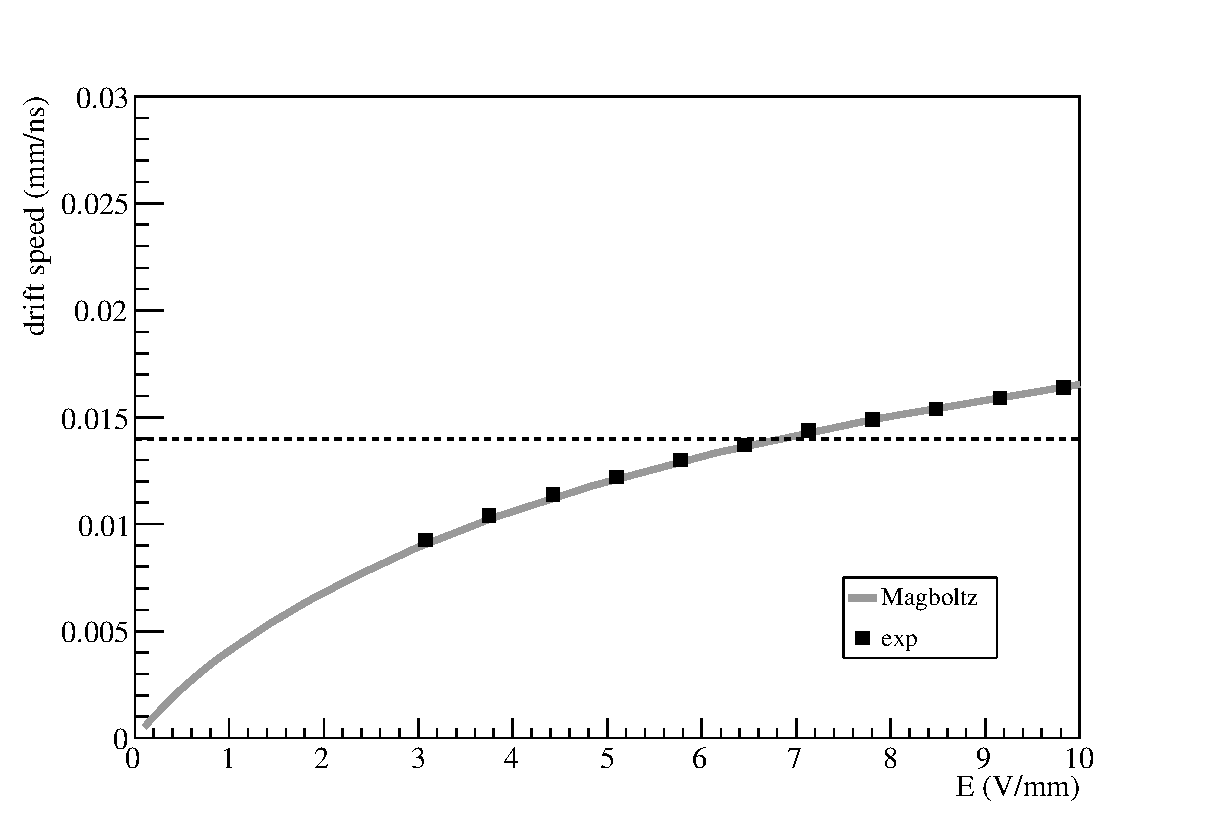
\includegraphics[clip, width=0.9\columnwidth]{eps/drift_v_iC4H10_H2.eps}
  \caption[検出ガスにiso-${\rm C_{4}H_{10}}$を用いたときのドリフトスピードの電場依存性。]
          {検出ガスにiso-${\rm C_{4}H_{10}}$を用いたときのドリフトスピードの電場依存性。
            図中の点線は0.014 mm/ns を示す。}
  \label{fig::drift_v_iC4H10_H2}
%  \includegraphics[clip, width=0.7\columnwidth]{eps/drift_v_iC4H10_He.eps}
  \caption{}
  \label{fig::drift_v_iC4H10_He}
\end{figure}
$\alpha$線源を用いて測定したドリフトスピードと Magboltz を用いて計算したドリフトスピードが一致していることが分かる。

\section{各種パラメータ}
\subsection{ドリフトスピード}
\subsection{ガス増幅率}
電圧パラメータを変更させたときの増幅率の変化を測定した。
増幅率を計算するためには荷電粒子が検出ガス中を通過した際に発生する電子数 ($N_{\rm e}$) と
増幅後に$\mu$-PICによって収集された電子数 ($N'_{\rm e}$) の比を取る。
$N_{\rm e}$はガス中での荷電粒子のエネルギー損失とガスのW値から求める。
$N'_{\rm e}$は$\mu$-PICで収集した電荷から求める。
詳しい計算方法について以下で述べる。

ガス中で荷電粒子がエネルギーを落とすと、W値あたり平均1個の電子を電離する。
そのため、荷電粒子のエネルギー損失をW値で割ることで$N_{\rm e}$が求まる。
各ガスのエネルギー損失とW値~\cite{energy_per_ion_pair,pdg}を表\ref{tab::energy_loss_and_W_val}に示す。
測定に用いた$\alpha$線源からは平均4.2 MeVの$\alpha$粒子が出ていることが他の測定によりわかっている。
エネルギー損失は4.2 MeVの$\alpha$粒子が$\mu$-PIC 32 strip分の距離 (12.8 mm) で落とすエネルギーを示している。
\begin{table}
  \centering
  \caption[検出ガスのW値とエネルギー損失と$N_{\rm e}$。]
          {検出ガスのW値とエネルギー損失と$N_{\rm e}$。
          エネルギー損失は荷電粒子がガス中を12.8 mm 進んだ時のものである。}
  \label{tab::energy_loss_and_W_val}
  \begin{tabular}{cccc}
    \toprule
    gas & W (eV) & energy loss (MeV) & $N_{\rm e}$\\
    \midrule
    ${\rm CH_{4}}$                          & 29.1 & 0.0565 & 1.94$\times 10^{3}$ \\
    ${\rm CH_{4} (3) + H_{2} (7)}$          & 34.2 & 0.0534 & 1.56$\times 10^{3}$ \\
    ${\rm CH_{4} (4) + He (7)}$             & 39.2 & 0.0593 & 1.51$\times 10^{3}$ \\
%    iso-${\rm C_{4}H_{10}}$                 & 26.0 & 0.0552 & 2.12$\times 10^{3}$ \\
    iso-${\rm C_{4}H_{10} (1) + H_{2} (9)}$ & 35.4 & 0.0620 & 1.75$\times 10^{3}$ \\
    iso-${\rm C_{4}H_{10} (1) + He (9)}$    & 44.0 & 0.0580 & 1.32$\times 10^{3}$ \\
    \bottomrule
  \end{tabular}
\end{table}

$\mu$-PICからの信号波形は32 strips まとめて図\ref{fig::FADC_waveform}のようなFADC情報として取得している。
この信号波形を時間で積分することによって32 strips で収集した電荷量を計算することができる。
$\mu$-PICで取得した電気信号は読み出し回路内部で800倍に増幅され、
入力インピーダンス50$\Omega$ で電流値を電圧値に変換して取得している。
よって、式 (\ref{eq::N'e})で求めることができる。
$e$は電荷素量である。
\begin{equation}
  N'_{\rm e} = \frac{\int V (t) dt}{ 50 \times 800 \times e}
  \label{eq::N'e}
\end{equation}

\subsubsection{GEMによるガス増幅}

\subsubsection{$\mu$-PICによるガス増幅}

\subsubsection{GEMとgrid間の電位差による電子の収集効率}

\subsection{幅}

\section{シミュレーションによる線源データの再現}
%\subsection{CH$_{\text 4}$}
%\subsection{CH$_{\text 4}$ + He}
%\subsection{CH$_{\text 4}$ + H$_{\text 2}$}
%\subsection{iso-C$_{\text 4}$H$_{\text 10}$ + He}
%\subsection{iso-C$_{\text 4}$H$_{\text 10}$ + H$_{\text 2}$}

\section{トリプルアルファ反応のシミュレーション}
%\subsection{CH$_{\text 4}$}
%\subsection{CH$_{\text 4}$ + He}
%\subsection{CH$_{\text 4}$ + H$_{\text 2}$}
%\subsection{iso-C$_{\text 4}$H$_{\text 10}$ + He}
%\subsection{iso-C$_{\text 4}$H$_{\text 10}$ + H$_{\text 2}$}
